% mainfile: ../../../../master.tex
\subsection{DNA and RNA quantification with NanoDrop\cR ND-1000 Spectrophotometer}
% The part of the label after the colon must match the file name. Otherwise,
% conditional compilation based on task labels does NOT work.
\label{task:20180301_cj1}
\tags{lab,dna,rna,qnt}
\authors{cj}
%\files{}
%\persons{}
\sidenote{While I measure the absorbance of my samples with the NanoDrop\cR ND-1000, I leave the Qubit\texttrademark kits at room temperature so it will be ready one I am done.}

\begin{figure}[H] % position of the figure 
    \centering
    \caption{NanoDrop spectra for DNA and RNA isolated with AllPrep Mini Kit}
    \label{fig:CJ20180301}
    \begin{subfigure}[b]{0.49\textwidth}
        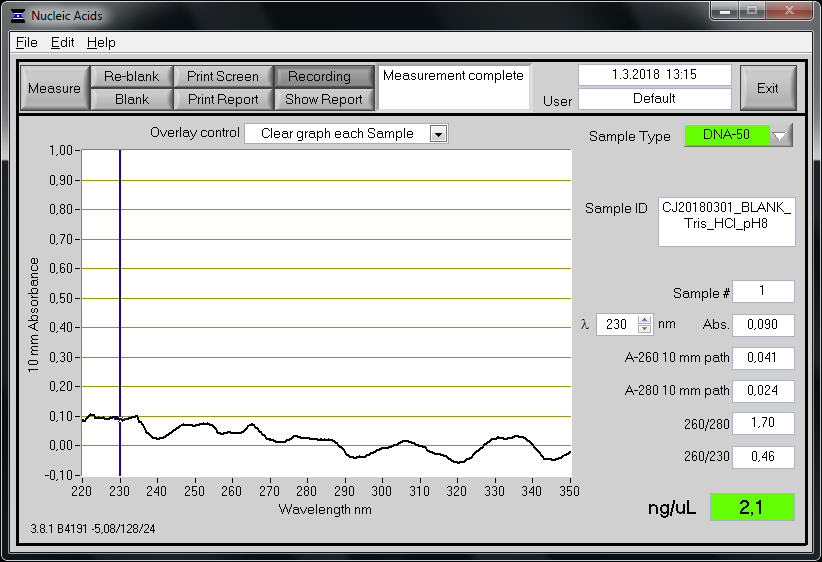
\includegraphics[width=\textwidth]{graphics/screenshots/CJ20180301_BLANK1.png}
        \caption{Spectrum of the Tris-HCl buffer pH 8 used as Blank: this blank is not acceptable and would lead to unaccurate measurments.}
        \label{sfig:CJ20180301_BLANK1}
    \end{subfigure}
    \\
    \begin{subfigure}[b]{0.49\textwidth}
        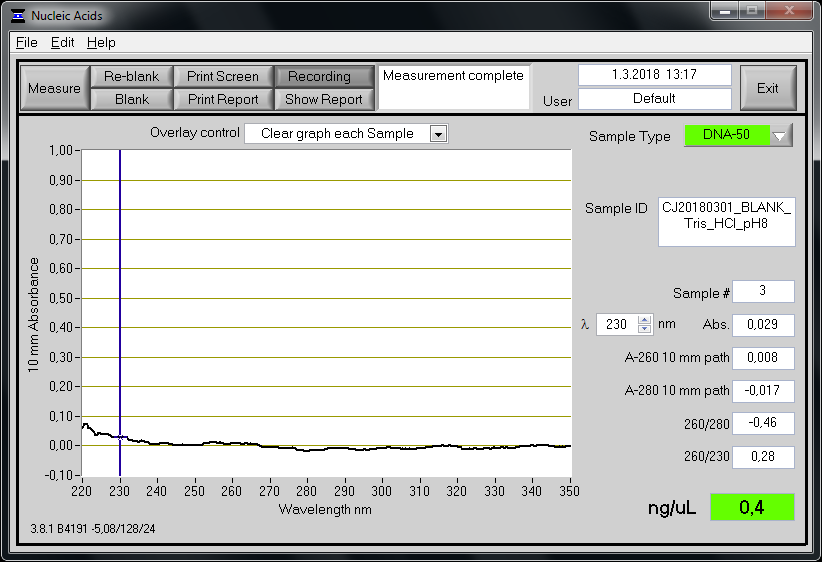
\includegraphics[width=\textwidth]{graphics/screenshots/CJ20180301_BLANK_Tris_HCl_pH8.png}
        \caption{Spectrum of the Tris-HCl buffer pH 8 used as Blank}
        \label{sfig:CJ20180301_BLANK_TrisHCl_pH8}
    \end{subfigure}
    ~ 
    \begin{subfigure}[b]{0.49\textwidth}
        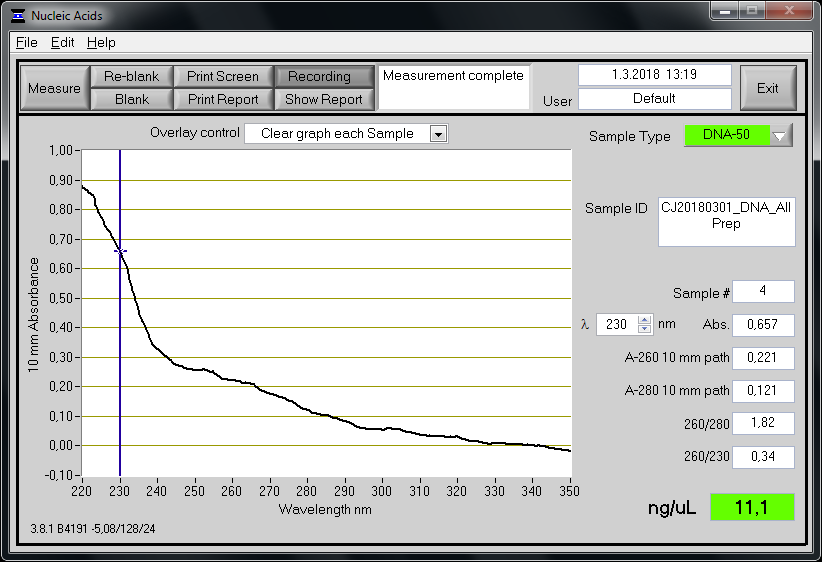
\includegraphics[width=\textwidth]{graphics/screenshots/CJ20180301_DNA_AllPrep.png}
        \caption{Spectrum of the DNA extracted with AllPrep}
        \label{sfig:CJ20180301_DNA_AllPrep}
    \end{subfigure}
    \\
    \begin{subfigure}[b]{0.49\textwidth}
        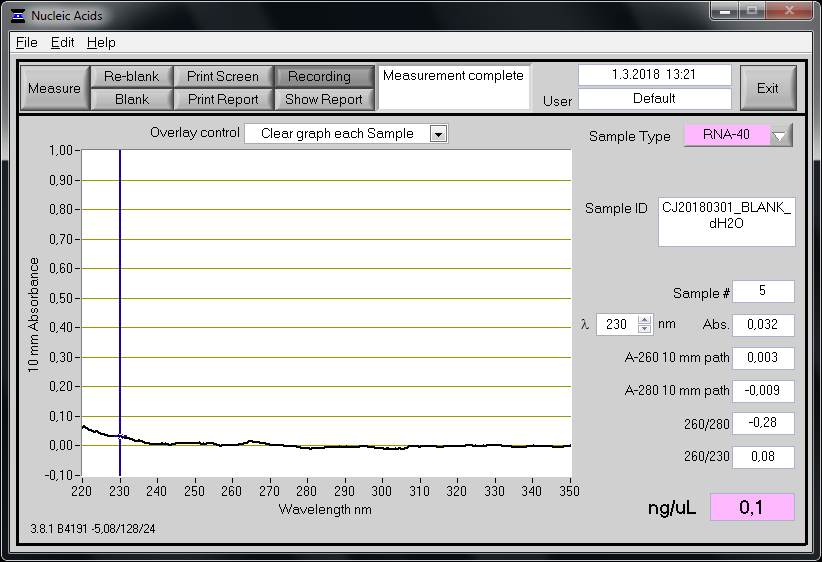
\includegraphics[width=\textwidth]{graphics/screenshots/CJ20180301_BLANK_dH2O.png}
        \caption{Spectrum of the dH2O used as Blank}
        \label{sfig:CJ20180301_BLANK_dH2O}
    \end{subfigure}
    ~ 
    \begin{subfigure}[b]{0.49\textwidth}
        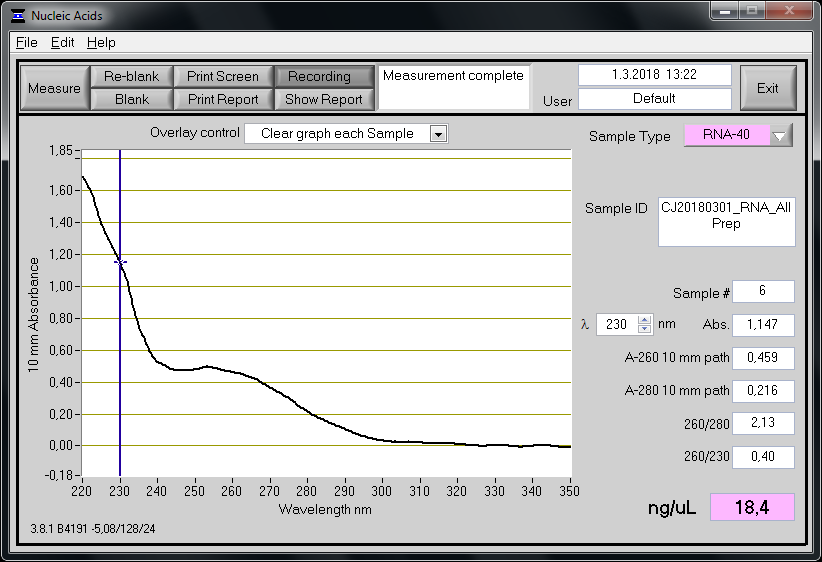
\includegraphics[width=\textwidth]{graphics/screenshots/CJ20180301_RNA.png}
        \caption{Spectrum of the RNA extracted with AllPrep}
        \label{sfig:CJ20180301_RNA_AllPrep}
    \end{subfigure}
\end{figure}

The spectra shown in figure \ref{fig:CJ20180301} are not good spectra but they are consistent with previous spectra obtained for nucleic acids isolated with the AllPrep Mini Kit by QIAGEN. 

\begin{table}[htbp]
\caption{res/nanodrop/CJ20180301.txt}
\label{tab:}
\centering
\begin{tabular}{l l l l l l l l l l l l l }
\toprule
Sample ID & Time  & ng/\uL  & A260  & A280  & 260/280  & 260/230  \\ \midrule
\texttt{CJ20180301\_BLANK\_Tris\_HCl\_pH8} & 13:15 & 2,07 & 0,041 & 0,024 & 1,70 & 0,46 \\
\texttt{CJ20180301\_BLANK\_Tris\_HCl\_pH8} & 13:16 & 4,61 & 0,092 & 0,049 & 1,88 & 1,60 \\
\texttt{CJ20180301\_BLANK\_Tris\_HCl\_pH8} & 13:17 & 0,40 & 0,008 & -0,017 & -0,46 & 0,28 \\
\texttt{CJ20180301\_DNA\_AllPrep} & 13:19 & 11,05 & 0,221 & 0,121 & 1,82 & 0,34 \\
\texttt{CJ20180301\_BLANK\_dH2O} & 13:21 & 0,11 & 0,003 & -0,009 & -0,28 & 0,08 \\
\texttt{CJ20180301\_RNA\_AllPrep} & 13:22 & 18,36 & 0,459 & 0,216 & 2,13 & 0,40 \\
\bottomrule
\end{tabular}
\\
User: Default - Date: 1.3.2018 - Constant: 40,00 - Cursor position: 230 \
\end{table}
